%!TEX root = ../thesis.tex
%*******************************************************************************
%*********************************** Seventh Chapter *****************************
%*******************************************************************************

\chapter{Research of the change of baseline impedance during proximal occlusion of the limb}  %Title of the First Chapter
\label{chapter occlusion}

\ifpdf
\graphicspath{{Chapter7/Figs/Raster/}{Chapter7/Figs/PDF/}{Chapter7/Figs/}}
\else
\graphicspath{{Chapter7/Figs/Vector/}{Chapter7/Figs/}}
\fi

\mynote{I have to change the captions of the graphs. They must be reviewed}
Venous occlusion plethysmography requires occluding the proximal section of the arm, obstructing the return of the venous blood.  This kind of examination is used to assess peripheral vascular diseases such as deep venous thrombosis.  In this study, the upper arm was occluded using a cuff at three different levels to recreate the effect of venous occlusion plethysmography.

As explained in chapter \ref{chapter procedure}, the experiment proceeds by recording five minutes of baseline signal followed by a level of occlusion. From there, regions 1, 3, 5 and 7 refer to the five minutes of baseline waveform. On the other hand, regions 2, 4 and 6 are equivalent to venous, partial arterial and total occlusions. In average the level of occlusion for each area were \SI{55}{\mmHg}, \SI{94.62}{\mmHg}, and  \SI{136.25}{\mmHg} respectively. Table  \ref{tbl:occlusions} describes the levels of occlusion for each participant. 

During the occlusion of the venous return in the upper arm, the blood pools within the veins in the forearm increasing its volume. This increase of volume reflects a change of resistivity as a more conductive medium is present. 

When the occlusion pressure is below diastolic occlusion, it is only affecting the blood return towards the hearth, but the arterial blood is still coming in the arm. In contrast, blocking the upper arm between diastolic and systolic pressures not only prevents the venous blood return but also constricts the income of arterial pressure into the arm. In the case of total occlusion when the cuff's pressure is above systolic pressure, both venous and arterial flows are blocked. 

This section described in detail the change of impedance in each region. Also, from the data obtained the estimation of blood flow is estimated.

\section{Change of basal impedance during occlusion}
\label{section occlusion 1}
From the data obtained in the experimental procedure, different data regions were extracted according to the kind of occlusion applied. The data were separated in this section into the readings from venous occlusion, partial arterial occlusion (PAO) and total blockage. 

The analysis of the data has to be performed only on the basal impedance. Similarly, as the previous chapter, the arterial pulses were eliminated from the signal. Only, the lower envelope of the impedance signal was used to perform this investigation. 

The data set for this study was subdivided as follows: two minutes of data before the occlusion as the baseline reference, then three minutes of occlusion followed by two minutes of data after releasing the cuff's pressure. 

\subsection{Changes of impedance during venous occlusion}
\label{section occlusion 1.1}
The basal impedance dropped while performing venous occlusion in each participant, as expected. As figure \ref{fig:venous statistics impedance} confirms, all the partakers experienced a decrease in their basal impedance during the region 2 of the experiment. The boxplot shows the three regions that took part of this part of the study. The data of the region 1 (\textit{R1}) were the last \SI{2}{\minute} of the initial baseline (\SIrange{180}{300}{\second}). Thereafter, it is the venous occlusion in region 2 (\textit{R2}) during \SI{3}{\minute} at the pressure levels describe by the column \textit{occlusion 1} in \ref{tbl: venous occlusions}, it is clear that the median resistance value decreased. Analysing this candle-stick can be described that the larger the distribution of the upper and lower quartile, the greater the resistance drop as registered by most of the participants, except participant 6 which impedance measurement settled quickly. After releasing the cuff's air, it was expected that the median impedance in region 3 would return to a value close to the initial baseline. However, partakers 3 and 4 did not recover completely. Indeed their resistance values improved for a few seconds but later on continue falling below the lower whisker of region 2. On the other hand, participants 1 rose over the initial baseline median. The only one showing a return to baseline was participant 3. 

\begin{figure}[htbp]
	\centering
	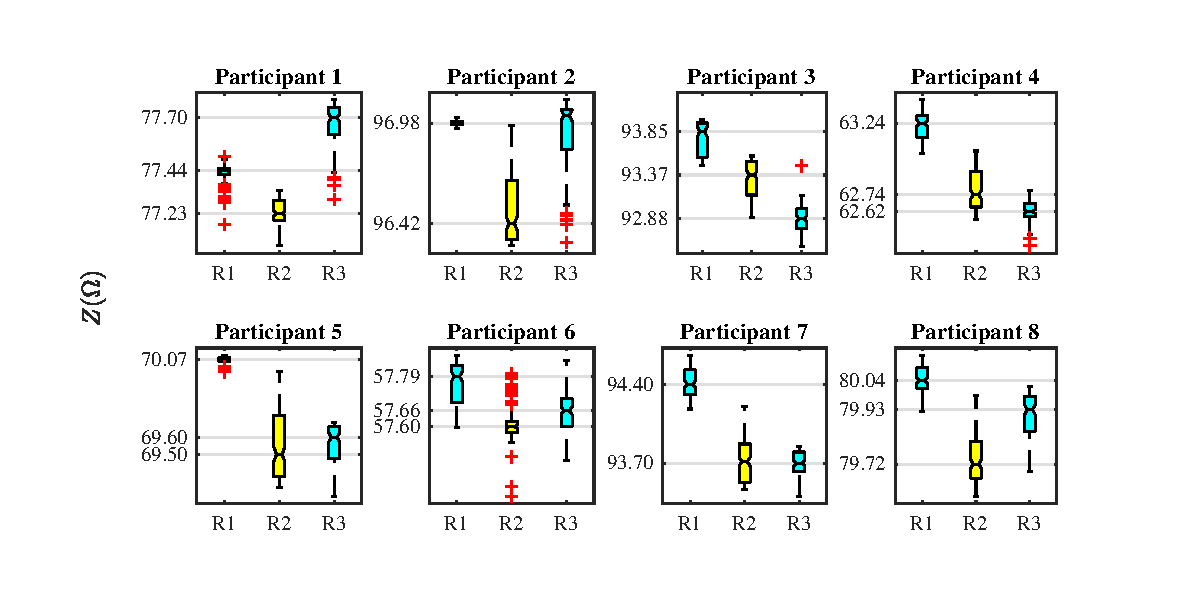
\includegraphics[width=15cm,keepaspectratio]{figure_vop_1}    
	\caption[Change of impedance during venous occlusion plethysmography]{Statistical change of impedance in $\Omega$ during venous occlusion plethysmography. The cyan boxplot represents the baseline before (Region 1) and after (Region 3) the occlusion. The yellow boxplot is the impedance during venous occlusion (Region 2).}
	\label{fig:venous statistics impedance}
\end{figure}  
 
Figure \ref{fig:venous occlusion impedance} shows the deviation of the impedance in terms of change in percentage of impedance ($\Delta Z\%$) from the median baseline in region 1. The shaded area represents the venous occlusion between \SIrange{300}{400}{\second}. The dots are the points of the foot of the signal equivalent to ($R_B$). The signal was smoothed using the command \textit{smooth} in Matlab which assigns a lower weight to outliers in the regression. This method assigns zero weight to data outside six mean absolute deviations \cite{MATLAB:2016}. Hence, it eliminates most of the rapid variations of impedance caused by motion artefact. 

\begin{figure}[htbp]
	\centering
	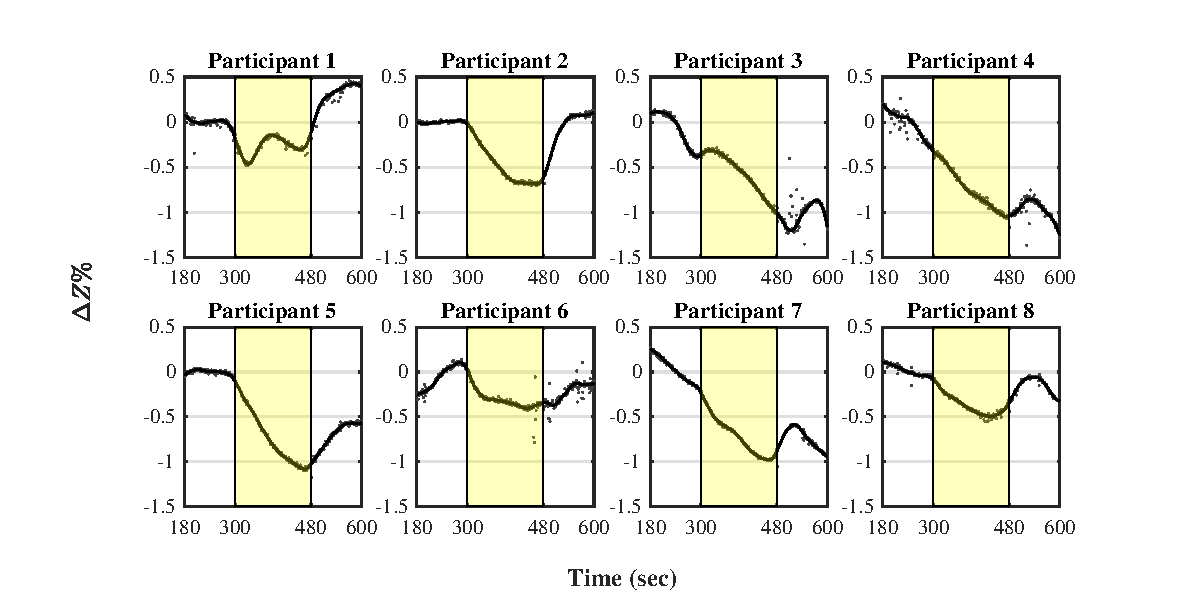
\includegraphics[width=15cm,keepaspectratio]{figure_vop_2}    
	\caption[Percentile variation of impedance during venous occlusion plethysmography]{Percentile change of impedance, using as reference average baseline impedance during the last \SI{2}{\minute} before the venous occlusion.}
	\label{fig:venous occlusion impedance}
\end{figure} 

The figure clearly reveals a linear trend during venous occlusion for most of the subjects. Nonetheless, participant's 1 resistance fell immediately as the occlusion occurred but a minute later, the participant moved his arm reversing the trend. Later on, the impedance continued decreasing again. Furthermore,  participant 6 also showed a similar response when the individual moved his arm, but in his case, the resistance settled instead of reversing the trend. Interestingly, participant 2 showed a saturation point after quite a few seconds, which it was particular of this subject. 

\mynote{Consult if callinf this $\Delta Z \%$ is a good name. I'd called it $\%_Z$ or $\%_\Omega$}

The table \ref{tbl:vop delta impedance} summarises the changes of impedance during the venous occlusion. The average median of the resistance drop from the baseline value was roughly \SI{-0.546(0076)}{\Delta \%}, where participants 4, 5 and 7 recorded the largest loss of impedance (>\SI{0.5}{\%}). The column \textit{Change} on the same table shows the impedance difference from the initial occlusion point to the minimum point of the smooth curve, calculated using equation \ref{eq:DeltaZ}. It revealed that during the venous occlusion the whole slope recorded a variation of \SI{0.658(0230)}{\percent}.

\begin{align}
	\label{eq:DeltaZ}
	\Delta Z\%_T = \Delta Z\%_{300 sec} - \Delta Z\%_{min}
\end{align}

 
\begin{table}[htbp]
	\caption[Statistical analysis of the percentile change of impedance during venous occlusion]{Statistical analysis of the percentile change of impedance during total occlusion. The data represents the median percentile change of impedance per participant, the maximum and minimum value of the occlusion and the difference between these two peak values.}
	\label{tbl:vop delta impedance}
	\centering
 	\begin{tabu}{l@{\hspace{1cm}}
 			     S[table-format=1.2]@{\,\( \pm \)\,}
 			     S[table-format=1.2]
 			     c
 			     c
 			     c}
 		\toprule
		&\multicolumn{2}{c}{\textbf{Median}}  
		&\textbf{Max} 
		&\textbf{Min}
		&\textbf{Change} \\ 
		&\multicolumn{2}{c}{\textbf{[$\Delta Z \%$]}}
		&\textbf{[$\Delta Z \%$]}
		&\textbf{[$\Delta Z \%$]}
		&\textbf{[$\Delta Z \%$]}\\\midrule
		Participant 1 & -0.26 & 0.09 & -0.20 & -0.47 & 0.26 \\ 
		Participant 2 & -0.58 & 0.21 & -0.03 & -0.69 & 0.66 \\  
		Participant 3 & -0.51 & 0.22 & -0.35 & -1.00 & 0.66 \\  
		Participant 4 & -0.79 & 0.22 & -0.32 & -1.06 & 0.74 \\ 
		Participant 5 & -0.82 & 0.30 & -0.11 & -1.09 & 0.98 \\  
		Participant 6 & -0.33 & 0.09 &  0.03 & -0.41 & 0.43 \\  
		Participant 7 & -0.72 & 0.22 & -0.22 & -0.98 & 0.77 \\  
		Participant 8 & -0.40 & 0.11 & -0.09 & -0.50 & 0.41 \\  
		\bottomrule
	\end{tabu} 
\end{table}		  
 
It is alluring to note the immediate change of impedance as soon as the venous occlusion occurs. The capability of impedance plethysmography device to detect venous  occlusion in all the participants is remarkable and almost instantaneous. As soon as the blockage occurs the impedance drops for some time, if motion does not change the trend, some could reached saturation as seen on participant 2. However, it is also apparent that other signals also reached a point of saturation, portraying a decrease of impedance in an exponential trend than linear. 

This effect can be summarised in figure \ref{fig:venous occlusion change}. This plot describes the change of impedance in time ($dZ/dt$) against some data points (beats) during the venous occlusion. For this, 10 data points of $R_B$, which are synchronised with the heart cycle, were clustered computing $dZ/dt$. This differential value is equivalent to the velocity of change of the basal impedance per second (\si{\ohm\per\second}). In general the average impedance all along the whole occlusion was \SI{-0.0026(00018)}{\beats}.

\begin{figure}[htbp]
	\centering
	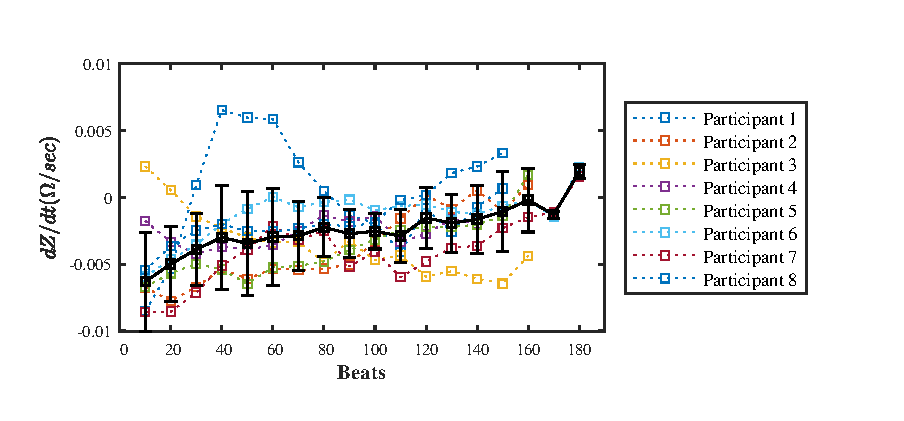
\includegraphics[width=15cm,keepaspectratio]{figure_vop_3}    
	\caption[Rate of change of impedance per 10 heartbeats during venous occlusion]{Speed of change of impedance in time per every 10 heartbeats. The colour lines represent the data per each participant. The dark bolded line is the mean of all the measurements.}
	\label{fig:venous occlusion change}
\end{figure}

From the figure can be concluded that during the first 10 beats, there is a higher drop of impedance compared to the last data points. Indeed, the rate of change of resistance in the first 10 beats was in average \SI{-0.0063(00037)}{\Omega\per\second}. After 90 beats the result of the derivation was more than halved to an average of \SI{-0.0027(00018)}{\Omega\per\second}. At 160 beats the ratio was reduced to just \SI{-0.0002(00024)}{\Omega\per\second}. The final data points (180 beats) showed a reversion of the trend (\SI{0.0019(0005)}{\Omega\per\second}). However, this is due to the just few participants achieved that amount of heart beats.  Moreover, at this point some data were already returning to baseline because the cuff could have been released few seconds earlier.  
 

%%********************************** % Section 7.1.2 ******************************************
\subsection{Change of impedance during partial arterial occlusion}
\label{section occlusion 1.2}
The same analysis performed on the VOP was applied to the partial arterial occlusion. The partial restriction of the arterial blood flow is achieved by mechanically occluding the upper arm between diastolic and systolic pressures. The load levels used to create these occlusions are detailed on the column \textit{occlusion 2} in the table \ref{tbl: venous occlusions}. Similar time lapses were used to analyse the data, the last \SI{2}{\minute} of the region 3 (\SIrange{660}{780}{\second}), the whole partial arterial blockage in region 4, \SI{3}{\minute} between \SIrange{780}{960}{\second}, followed by \SI{2}{\minute} of return to baseline after releasing the pressure of the cuff in region 5 (\SIrange{960}{1080}{\second}).

Occluding the blood flow at this pressure level induced an uncomfortable feeling on the participants, some of them felt numbness in their arms during the study. Therefore, some partakers moved their arms like participant 1, in others, the length of the occlusion had to be shortened like in participant 4 where the occlusion occurred later (\SIrange{840}{960}{\second}) because ECG sensors had to be relocated and participant 8 who asked to terminate the blockage a minute earlier (\SIrange{780}{900}{\second}). 

During this kind of occlusion, there is no venous return, as well as the inflow being slightly restricted. Indeed, the occlusion constricts the brachial artery where only a  small amount of blood passes through the obstruction. Moreover, the blood flow becomes turbulent after the cuff's constriction.  Due to the venous occlusion action, it is expected the arm to increase its volume as blood pools in the forearm reducing the basal impedance. 

Figure \ref{fig:partial arterial statistics impedance} confirms the reduction of the basal impedance all along partial arterial occlusion. Comparable to VOP, the box-plot shows a larger upper and lower quartile distribution for most of the participants in region 4, because of a continued drop in basal impedance during that occlusive action. However, partaker 4 depicted a significant number of outliers, which was mainly caused by motion artefact. The data also reports that only a few participants were able to get back close to baseline resistance, such as participants 2 and 7. Interestingly, some study members displayed a swift recovery in the region 5. For instance, the large data distribution in participants 1, 2, 4, 6, 7 and 8 describes a fast trend to return to baseline. But in general terms, it seems that a longer recovery time is required to return to an impedance value close to baseline after partial arterial occlusion. 

\begin{figure}[htbp]
	\centering
	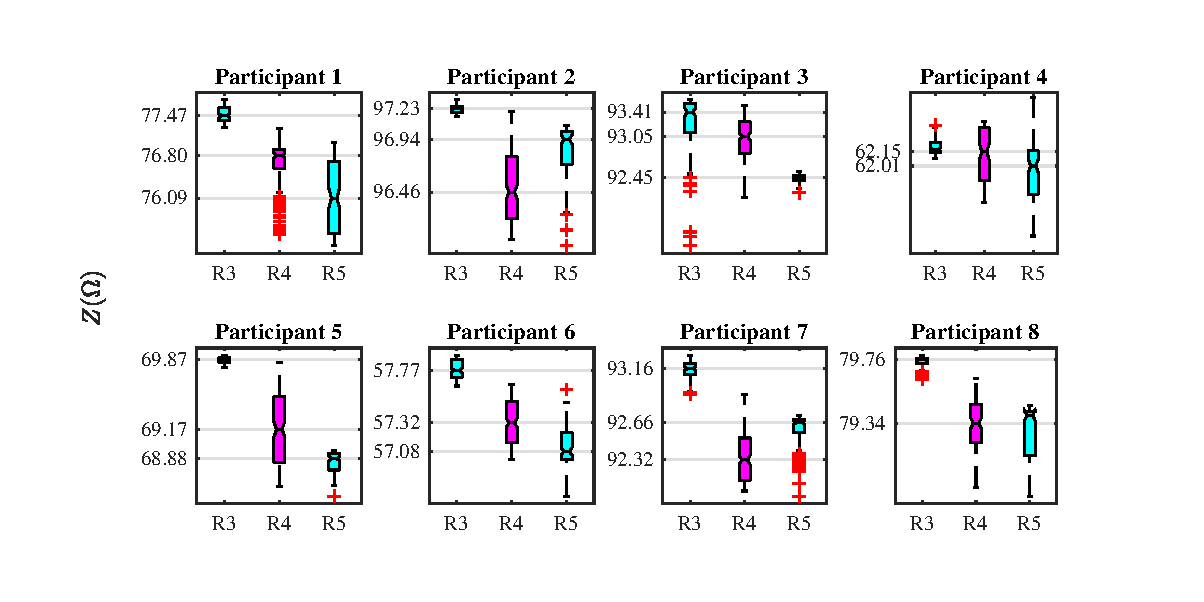
\includegraphics[width=15cm,keepaspectratio]{figure_vop_4}    
	\caption[Change of impedance during partial arterial occlusion]{Statistical change of impedance in $\Omega$ during partial arterial occlusion. The cyan boxplot represents the baseline before (Region 3) and after (Region 5) the occlusion. The magenta boxplot is the impedance during partial arterial occlusion (Region 4).}
	\label{fig:partial arterial statistics impedance}
\end{figure}  

By qualitatively analysing the change of impedance by percentage from baseline region 3, figure \ref{fig:arterial occlusion imepdance} displays that there is a linear trend during the cuff's pressure in the region 4. Certainly, it can be noticed that the impedance drop is more pronounced than the one from venous occlusion (see figure \ref{fig:venous occlusion impedance}). In participant 1 the motion artefact is more evident, the step drop of basal impedance right before the release of the cuff's pressure is a reflection of the muscular movement of his forearm. In this case, it is evident that the arm movement augmented the change of impedance throughout the occlusion. However, other participants also experienced motion artefact, but the change of impedance was just within a few heart beats. For instance, participant 2 showed only a data point off the smooth line, but in participants 3 and 4, the amount of data points off the soft signal were significantly larger. But in summary, most of the participants described a straight drop of impedance, especially linear in participants 2 and 5. 

After releasing the cuff's pressure, it is easy to see that most of the signals change the slope of the signal. The only one that did not reflect this change was participant 3. This impedance correction reflects the restoration of the blood circulation and the reduction of the forearm's volume. Moreover, there is not an apparent settling impedance value, except for participant 7 and 8. In general, this change of trend also confirms that the body might require longer to recover after the partial arterial occlusion.

\begin{figure}[htbp]
	\centering
	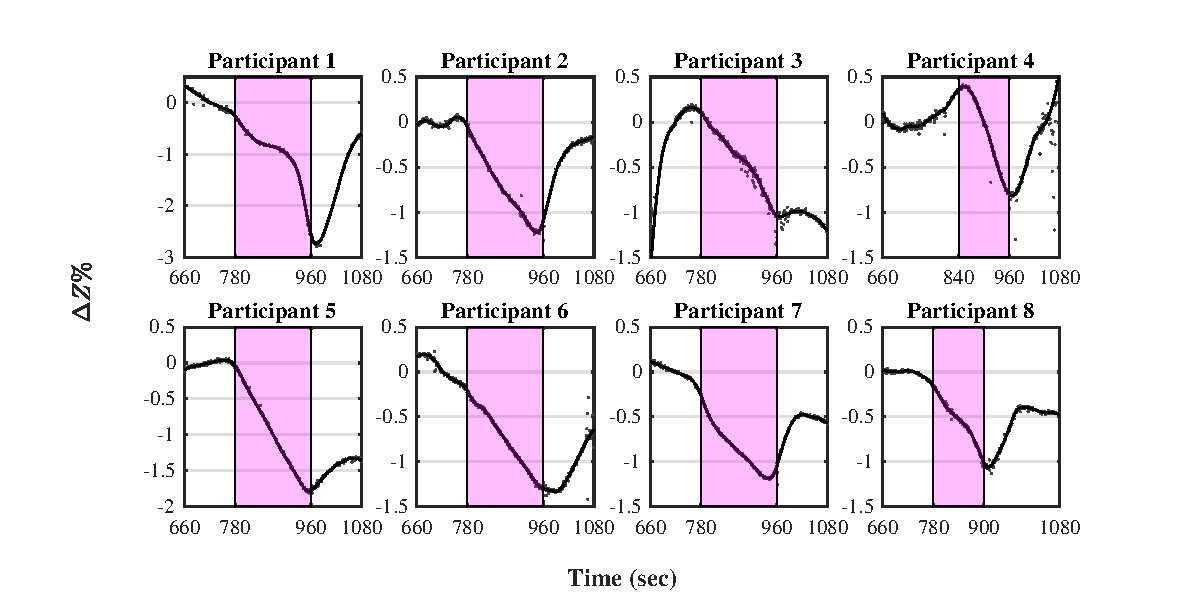
\includegraphics[width=15cm,keepaspectratio]{figure_vop_5}    
	\caption[Percentile variation of impedance during partial arterial occlusion]{Percentile change of impedance, using as reference average baseline impedance during the last \SI{2}{\minute} before the partial arterial occlusion.}
	\label{fig:arterial occlusion imepdance}
\end{figure}  

Table \ref{tbl:AO delta impedance} reports the percentage variations from the baseline impedance in region 3 in more depth. The median impedance drop from the baseline was approximately \SI{-0.783(0324)}{\percent}. However, participant 4 showed a lower median value, because of the initial impedance value was above the baseline average at \SI{0.34}{\percent}. Evidently, there is a larger reduction of impedance or increase of the forearm's volume rather than VOP. The median change of impedance from the maximum to the minimum value was around \SI{1.133(0482)}{\percent} which is nearly double when compared to venous occlusion. A  physiological response might have caused this increase in volume. The blood pooling could not cause this increase of volume because the arterial blood flow was restricted, so less amount blood entered into the forearm segment. 

\begin{table}[htbp]
	\caption[Statistical analysis of the percentile change of impedance during partial arterial occlusion]{Statistical analysis of the percentile change of impedance during partial arterial occlusion. The data represents the median percentile change of impedance per participant, the maximum and minimum value during the occlusion and the difference between these two peak values.}
	\label{tbl:AO delta impedance}
	\centering
	\begin{tabu}{l@{\hspace{1cm}}
			S[table-format=1.2]@{\,\( \pm \)\,}
			S[table-format=1.2]
			c
			c
			c}
		\toprule
		&\multicolumn{2}{c}{\textbf{Median}}  
		&\textbf{Max} 
		&\textbf{Min}
		&\textbf{Change} \\ 
		&\multicolumn{2}{c}{\textbf{[$\Delta Z \%$]}}
		&\textbf{[$\Delta Z \%$]}
		&\textbf{[$\Delta Z \%$]}
		&\textbf{[$\Delta Z \%$]}\\\midrule
		Participant 1 & -0.85 & 0.50 & -0.28 & -2.56 & 2.29 \\  
		Participant 2 & -0.80 & 0.35 & -0.05 & -1.23 & 1.18 \\  
		Participant 3 & -0.38 & 0.32 &  0.10 & -1.04 & 1.14 \\  
		Participant 4 & -0.03 & 0.41 &  0.34 & -0.78 & 1.13 \\  
		Participant 5 & -1.01 & 0.54 & -0.04 & -1.80 & 1.76 \\  
		Participant 6 & -0.77 & 0.33 & -0.21 & -1.30 & 1.09 \\  
		Participant 7 & -0.90 & 0.26 & -0.25 & -1.19 & 0.93 \\  
		Participant 8 & -0.53 & 0.22 & -0.15 & -1.01 & 0.85 \\  
		\bottomrule
	\end{tabu} 
\end{table}	

\begin{figure}[!b]
	\centering
	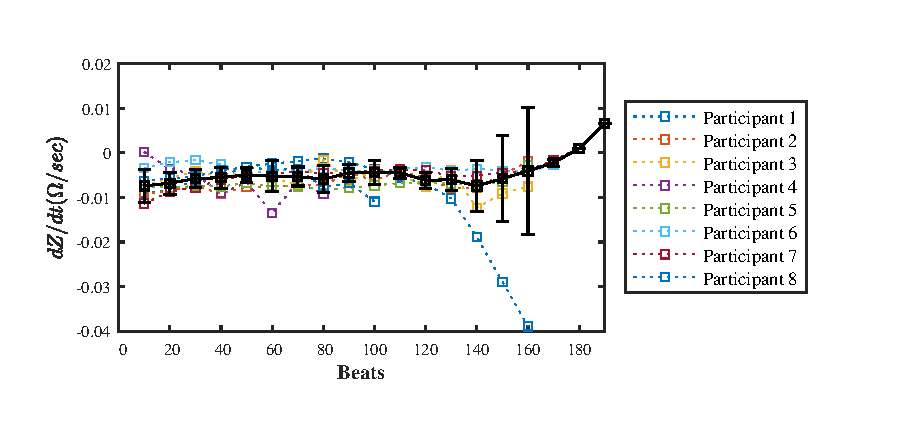
\includegraphics[width=15cm,keepaspectratio]{figure_vop_6}    
	\caption[Rate of change of impedance per 10 heartbeats during partial arterial occlusion]{Speed of change of impedance in time per every 10 heartbeats. The colour lines represent the data per each participant. The dark bolded line is the mean of all the measurements.}
	\label{fig:arterial occlusion change}
\end{figure}  

The calculation of the velocity of the change of impedance  ($dZ/dt$) displayed a similar exponential response as in VOP. Figure \ref{fig:arterial occlusion change} shows the calculation of these points for all the participants. The plot indicates that the first 10 beats of changed on a ratio average of \SI{-0.0074(00037)}{\Omega\per\second} which was the largest acceleration. Then between 20 and 110 beats the velocity stabilised to \SI{-0.0053(00007)}{\Omega\per\second}. After this apparent settling, there is a new increase in the differentiation. However, it seems to be aided by the motion artefact seen on participant 1 for a few beats. \mynote{Check if I can use time instead of beats}




%%********************************** % Section 7.1.3 ******************************************
\subsection{Impedance variation during total occlusion}
\label{section occlusion 1.3}
The blood supply towards the forearm was completely blocked by inflating the cuff above systolic pressure, in the case of this study \SI{20}{\mmHg} above this point. The column \textit{occlusion 3} in the table \ref{tbl: venous occlusions} shows the pressure level applied for the research. The data regions involved in this part of the investigation were regions 5, 6 and 7. Equally to previous occlusions analysis, the last 2 minutes of data from region 5 were used as impedance baseline (between \SIrange{1140}{1260}{\second}). Then, the cuff was inflated to accomplish complete blood flow obstruction; the occlusion was maintained for \SI{3}{\minute} between \SIrange{1260}{1440}{\second}. Finally, the cuff's air was immediately released, and readings were taken for further \SI{2}{\minute}.

This test caused a lot of discomfort to most of the participants, numbness and willingness to move their limb was common for all the participants. Hence, they ended up moving their arms voluntarily. Because there is no either blood flowing or pooling during this part of the experiment, it was expected small impedance variations. Additionally, the mean restive value would be equivalent to the impedance of the tissue's components within the segment plus the impedance of the residual blood in the forearm. However, when a change of resistivity happens, this is mostly caused by the participant's re-accommodation rather than a physiological variable. 

Figure \ref{fig:total arterial statistics impedance} shows how the impedance change during the total occlusion. Initially, it can be seen that there was not a consensus on the signal trend all along the occlusion as seen on the previous tests.  Some of the participants reflected a small reduction in their median impedance, like study members 1,  4, 5, 6 and 8, whereas the rest experienced a slight increase of it. Also, the trend of the signal during the occlusion is not clear; different signals have different data distribution points, for instance,  participant 1 and 7 displayed a large data distribution indicating a constant change of their median impedance. On the other hand, the rest showed a data distribution centred in the median, illustrating a little impedance variation during the occlusion. Only participant 5 exhibited a significant number of outliers, representing rapid changes at one point of the measurement. In general, there is not a linear trend as reported by the other kind of occlusions. 

After releasing the cuff's pressure, again there is not a definite trend in the direction of the impedance. Some of the participants displayed an increase of their resistivity. However, participants 4 and 5 presented exaggerated impedance changes. It is not clear the nature of this rare variation, but it could be due to the limb movement after the occlusion. Moreover, there is not a quick change of impedance as experienced on the other type of occlusions. Which, somehow is congruent with the fact that there is no blood rushing in or out of the forearm.

\begin{figure}[htpb]
	\centering
	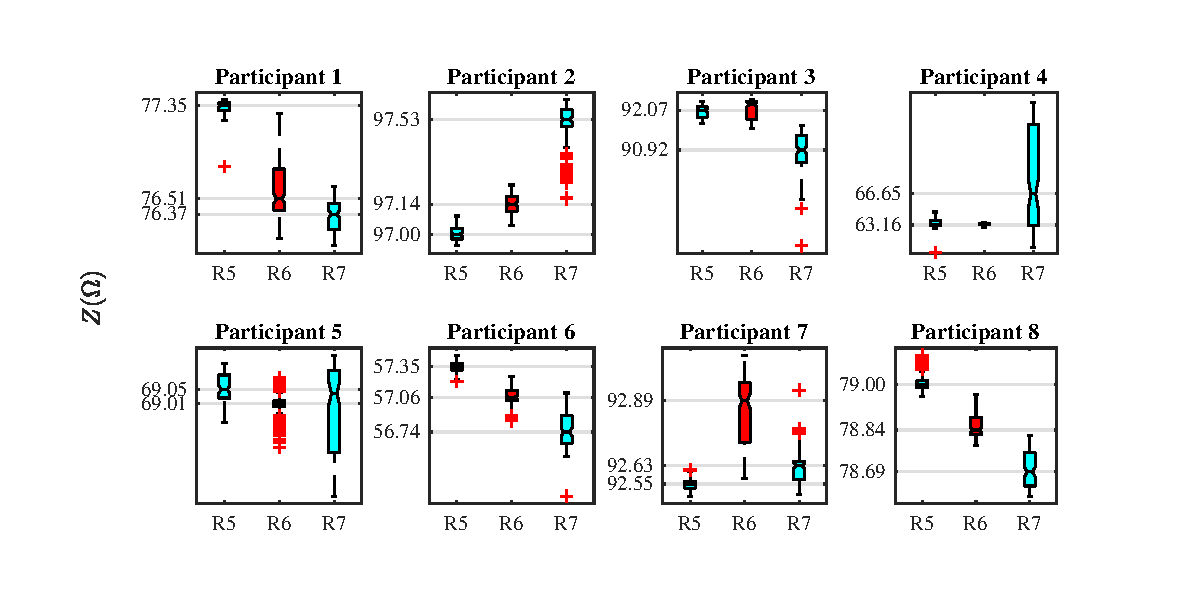
\includegraphics[width=15cm,keepaspectratio]{figure_vop_7}    
	\caption[Change of impedance during total occlusion]{Statistical change of impedance in $\Omega$ during total occlusion. The cyan boxplot represents the baseline before (Region 5) and after (Region 7) the occlusion. The red boxplot is the impedance during total occlusion (Region 6).}
	\label{fig:total arterial statistics impedance}
\end{figure} 

By analysing the variation of impedance during the occlusion compared to the baseline (region 5), it can be seen the magnitude and direction of the resistivity change. Evidently, participant 1 displayed the largest and continuous impedance decrease which is unusual for this type of occlusion. Another unexpected resistivity response was the one performed by participant 7 where his impedance increased in a small proportion.  

The table \ref{tbl:TO delta impedance} describes in detail the impedance changes during the occlusion. The median impedance during total occlusion was \SI{0.0427(04790)}{\percent} which is quite close to zero. However, the sign of column \textit{median} indicates that five out of eight exhibited a negative trend in the impedance direction, indicating resistivity loss. In fact, most of the measurements were below \SI{0.5}{\percent}, only participants 1 and 5 showed the higher changes of impedance. By calculating the $\Delta \%$  from the maximum and minimum changes (column \textit{Change}) can be deducted that only participant 1 presented a change greater than \SI{1}{\percent}, between \SIrange{0.5}{1}{\percent} participant 3 and 6 displayed this data range and the rest were below \SI{0.5}{\percent}. In general, the changes described by total occlusion were significantly lower than the other occlusions indicating a minimum increase of volume, for instance partakers 2 and 5 median impedance were a clear illustration of this. Some changes of impedance were presented in some measurements which can be related to a muscular activity. 

\begin{figure}[htbp]
	\centering
	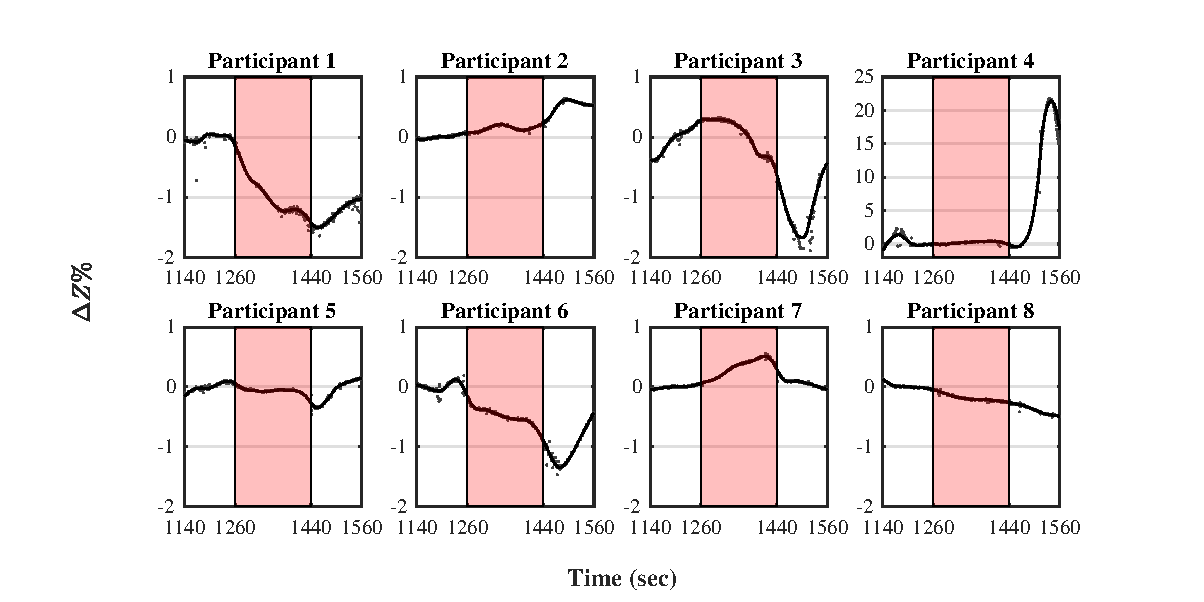
\includegraphics[width=15cm,keepaspectratio]{figure_vop_8}    
	\caption [Percentile variation of impedance during total occlusion]{Percentile change of impedance, using as reference average baseline impedance during the last \SI{2}{\minute} before the total occlusion.}
	\label{fig:total occlusion imepdance}
\end{figure} 

\begin{table}[htbp]
	\caption[Statistical analysis of the percentile change of impedance during total occlusion]{Statistical analysis of the percentile change of impedance during total occlusion. The data represents the median percentile change of impedance per participant, the maximum and minimum value during the occlusion and the difference between these two peak values.}
	\label{tbl:TO delta impedance}
	\centering
	\begin{tabu}{l@{\hspace{1cm}}
			S[table-format=1.2]@{\,\( \pm \)\,}
			S[table-format=1.2]
			c
			c
			c}
		\toprule
		&\multicolumn{2}{c}{\textbf{Median}}  
		&\textbf{Max} 
		&\textbf{Min}
		&\textbf{Change} \\ 
		&\multicolumn{2}{c}{\textbf{[$\Delta Z \%$]}}
		&\textbf{[$\Delta Z \%$]}
		&\textbf{[$\Delta Z \%$]}
		&\textbf{[$\Delta Z \%$]}\\\midrule
		Participant 1 & -1.09 & 0.33 & -0.14 & -1.38 & 1.24 \\  
		Participant 2 &  0.14 & 0.04 &  0.07 &  0.07 & 0.00 \\  
		Participant 3 &  0.18 & 0.28 &  0.30 & -0.50 & 0.81 \\  
		Participant 4 &  0.21 & 0.16 &  0.05 & -0.14 & 0.19 \\  
		Participant 5 & -0.06 & 0.05 &  0.05 & -0.23 & 0.28 \\  
		Participant 6 & -0.51 & 0.14 & -0.15 & -0.89 & 0.75 \\  
		Participant 7 & -0.36 & 0.15 &  0.05 &  0.05 & 0.00 \\  
		Participant 8 & -0.21 & 0.06 & -0.05 & -0.27 & 0.22 \\  
		\bottomrule
	\end{tabu} 
\end{table}	

Figure \ref{fig:total occlusion change} illustrates the analysis of the velocity rate ($dZ/dt$) which the basal impedance changes. It clearly reflects that participant 1 basal impedance decreased swiftly compared to the rest of the partakers. Also, participant 3 experienced a quick impedance drop between \SIrange{80}{140}{\beats}. In general, the average velocity for the total occlusion was around \SI{-0.00061(000170)}{\Omega\per\second} which is considerably small compared to the other occlusions. However, at the beginning of the occlusion, there was a modest increase in the velocity, the average for the first \SI{10}{\beats} was around \SI{-0.0027(00052)}{\Omega\per\second}. After that, it stabilised close to the median value of all the measurements until \SI{140}{\beats}. Nonetheless, between \SIrange{140}{180}{\beats} there was an increase in the velocity due to the contribution of the negative trends before releasing the occlusion. 

\begin{figure}[htbp]
	\centering
	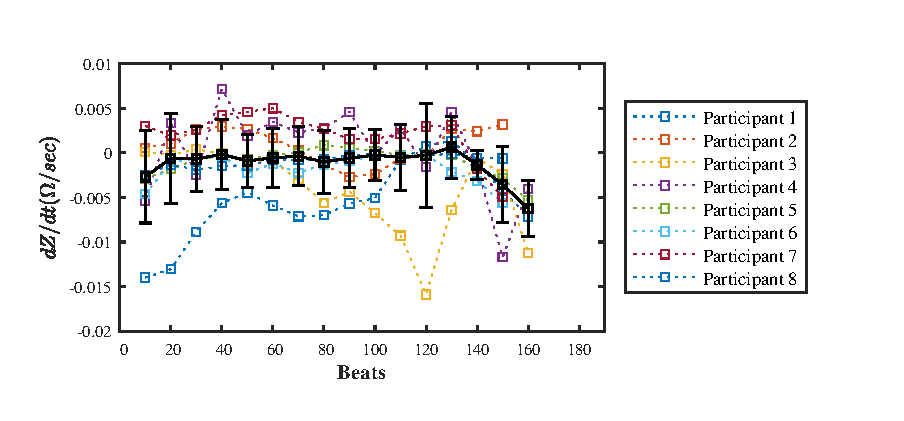
\includegraphics[width=15cm,keepaspectratio]{figure_vop_9}    
	\caption[Rate of change of impedance per 10 heartbeats during total occlusion]{Speed of change of impedance in time per every 10 heartbeats. The colour lines represent the data per each participant. The dark bolded line is the mean of all the measurements.}
	\label{fig:total occlusion change}
\end{figure} 


%%********************************** % Section 7.2 ******************************************


\section{Blood flow calculation from basal signal}
\label{section occlusion 2}
As the literature remarked in section \ref{section procedure 4}, it is possible to calculate the blood flow from the changes in the baseline impedance. When an arm is occluded at any point above venous pressure ($\approx$ \SI{25}{\mmHg}), an increase of volume in time occurs which is directly proportional to the blood flow coming into the distal section of the arm. Using the mathematical equations described in \ref{section procedure 4.1} is possible to convert the basal impedance into blood flow, if the distance between the sensing electrodes and the circumference of the forearm at these same points are known. Indeed, all this data is available from the experiment. Therefore, it is possible to quantify the blood flow during an occlusive event.  

From the equation \ref{eq:QL} \mynote{Verify if this is the correct equation. I'm using 5.18 with the square of $(L/RB)^2$} can be seen that the difference in impedance $\Delta R = R_{B2} - R_{B1}$ produces the sign of the mathematical equation. As it has been described, the resistance of the forearm drops when a venous occlusion occurs within a period of time $\Delta t$. Hence, a negative slope is produced during the changing impedance when $R_{B1} > R_{B2}$ resulting in a negative sign for the equation. Figure \ref{fig:relation R vs t} describes the expected relation between $\Delta R$ and $\Delta t$ when impedance is decreasing. On the contrary, if the slope of the change of impedance were positive then the sign of the equation would be positive. The sign, in this case, is only an indication of the direction of the blood flow \mynote{Find the reference where describes that the sign only indicates the direction}. If there is an increment on the impedance, it might be mainly caused by motion or other external variable but is not related to blood flow. For this reason, only the negative slope measurements are significant for the calculation of blood flow.

\begin{figure}[!htpb]
	\centering
	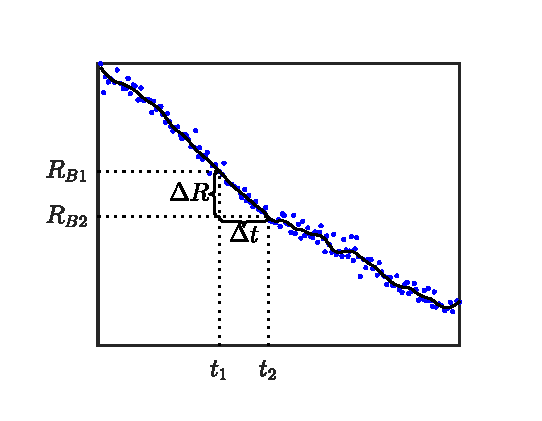
\includegraphics[width=9cm,keepaspectratio]{figure_vop_13}    
	\caption[Points for the calculation of the flow]{Points for the calculation of the flow between 2 points, $\Delta R = R_{B2} - R_{B1}$ and $\Delta t = t_2 - t_1$.}
	\label{fig:relation R vs t}
\end{figure}

From this principle, an algorithm was designed to calculate the blood flow within $n$ heart beats, only when a decrease of impedance is detected. From this, $\Delta R$ was calculated by getting the difference between the impedance in the tenth heartbeat and the first one ($R_{B(10)} - R_{B(1)}$).  Similarly, the $\Delta t$ was calculated From this principle, an algorithm was designed to calculate the blood flow within n heart beats, only when a decrease of impedance is detected. From this, $\Delta R$ was calculated by getting the difference between the impedance in the tenth heartbeat and the first one ($R_{B_{t=10}} - R_{B_{t=1}}$).  Similarly, the $\Delta t$ was calculated as the difference in time between the  \nth{1} and \nth{10} heartbeat ($t_{(t=10)} - t_{(t=1)}$). The value used to compute $R_B$ was equivalent to the value on the tenth heartbeat ($R_B = R_{B_{t=10}}$). The heart rate was calculated from the average difference of time of all the heartbeat detected.

\begin{equation}
\label{eq:QL}
\dot{Q} = \frac{60}{f_s}*\Bigg[\frac{1}{n}*\sum_{i=1}^{n}(t_{i+1} - t_{i}) \Bigg] * \rho * \Bigg( \frac{l}{R_{B_{t=n}}} \Bigg) ^2 *\Bigg(\frac{R_{B_{t=n}}-R_{B_{t=1}}}{t_{n}-t_{1}}\Bigg)
\end{equation}

\mynote{I'm trying to describe the algorithm in mathematics. I'm not completely sure that is correct. But describes the algorithm used}

Where $f_s$ is the sampling frequency of the original signal, $n$ are the number of heartbeats to be computed, $R_B$ is the basal impedances at difference time instances. One when $t=n$ equivalent to the time when $n$ heartbeat happened and $t=1$ the initial point in time for the calculation. 

%********************************** % Section 7.2.1 ******************************************
\subsection{Blood flow calculation using venous occlusion plethysmography}
\label{section occlusion 2.1}
The first calculation of blood flow will be performed with the data obtained all along venous occlusion plethysmography (VOP) during the time frame between \SIrange{300}{480}{\second}. Figure \ref{fig:blood_flow:venous_occlusion} displays on the left the smoothed impedance, which diminishes the effect of respiration and muscular activity in the signal. Indeed, this plot also shows additional information. First, the dots represent the instant points when a valley occurs, equivalent to a point where a heartbeat takes place. It must be remembered, that the dynamic component of the signal is synchronised with the cardiac cycle. The signal was smooth to avoid abrupt changes in resistivity. Also, the red markers indicate the initial point $t=1$ where the blood flow calculation takes place and the blue marker where it finishes $t=n$. For this data analysis, 10 heartbeats ($n=10$) were used to calculate the blood flow.

\begin{figure}[!htpb]
	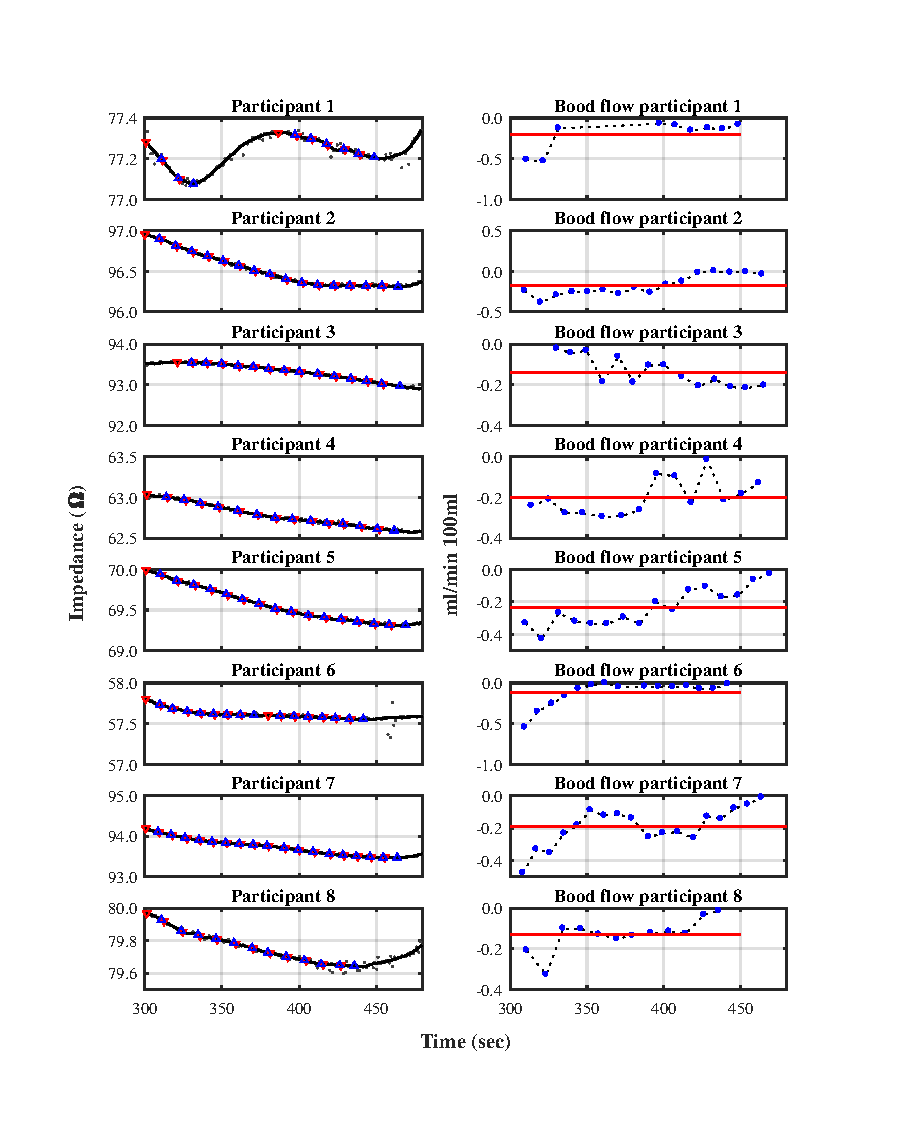
\includegraphics[width=\textwidth,height=\textheight,keepaspectratio,trim={0.5cm 0cm 0cm 1cm},clip]{figure_vop_10}    
	\caption[Blood flow calculated from venous occlusion plethysmography for every 10 beats of data points]{The figure on the left shows the change of impedance during venous occlusion plethysmography (\SIrange{300}{480}{\second}). The dots shows the valley points synchronised with the heart cycle. The dark line represents the smoothed data that used to calculate blood flow. The red marker indicates the initial data point $R_{B1}$ and the blue one $R_{B2}$. On the rights, the blood flow in \si{\bfv} for the data points between each marker. The red line indicates the mean of the data points.}
	\label{fig:blood_flow:venous_occlusion}
\end{figure}

As a result, the figure on the left of \ref{fig:blood_flow:venous_occlusion} was generated. Here, the blue points indicate the blood flow every $n=10$ points, only when the impedance's slope is negative. Besides, the red line shows the average blood flow for all the measurements during the experiment. The blood flow was calculated in units of \si{\bfv}. As it was anticipated, there is a greater change of blood flow when the difference $\Delta R$ takes place. As it can be noticed, when the signal gets close to a saturation point ($Delta R = \SI{0}{\Omega}$), the blood flow tends to zero. 

The table \ref{tbl:blood_flow:region2} shows a review of the data collected. The participant 1, only displayed 9 data points as the changing of direction was not count in the flow calculation. In general terms, the average calculated blood flow was \SI{-0.174(0042)}{\bfv}. Participant 6 was the only one that showed a blood flow close to zero (\SI{-0.001}{\bfv}) when reached a saturation point. The rest of the participants showed a maximum blood flow of < \SI{-0.010}{\bfv}.

\begin{table}[!htpb]
	\caption{Statistics of the blood flow calculated during venous occlusion. All the numbers are in blood flow units \si{\bfv}, except the column size that is the magnitude of sample.}
	\label{tbl:blood_flow:region2}
	\centering
	\begin{tabular}
		{
			l
			c
			c
			S[table-format=1.3]@{\,\( \pm \)\,}S[table-format=1.3] %Format for Z+-std 
			c
			c
		}
		\toprule
		& \multirow{2}{*}{\textbf{Size}} 
		& \textbf{Median} 
		& \multicolumn{2}{c}{\textbf{Mean}} 
		& \textbf{Max} & \textbf{Min} \\
		& 
		& \small{\si{[\bfv]}} 
		& \multicolumn{2}{c}{\small{\si{[\bfv]}}} 
		& \small{\si{[\bfv]}} 
		& \small{\si{[\bfv]}} \\\midrule
		Participant 1 & 9  & -0.129 & -0.204 & 0.184 & -0.070 & -0.535 \\ 
		Participant 2 & 15 & -0.232 & -0.186 & 0.118 & -0.010 & -0.386 \\ 
		Participant 3 & 15 & -0.161 & -0.138 & 0.070 & -0.022 & -0.216 \\ 
		Participant 4 & 15 & -0.214 & -0.196 & 0.086 & -0.015 & -0.296 \\ 
		Participant 5 & 16 & -0.259 & -0.235 & 0.115 & -0.028 & -0.428 \\ 
		Participant 6 & 16 & -0.051 & -0.113 & 0.150 & -0.001 & -0.547 \\ 
		Participant 7 & 18 & -0.164 & -0.191 & 0.117 & -0.012 & -0.476 \\ 
		Participant 8 & 12 & -0.125 & -0.131 & 0.080 & -0.013 & -0.328 \\ 
 \bottomrule
	\end{tabular} 
\end{table}


%********************************** % Section 7.2.2 ******************************************
\subsection{Blood flow calculation during partial arterial occlusion}
\label{section occlusion 2.2}

Similar to the blood flow calculated during VOP, the blood flow during partial arterial was calculated (between \SIrange{780}{960}{\second}). As section \ref{section occlusion 1.2} described, the impedance slope during partial arterial occlusion was nearly doubled when compared to venous occlusion. Therefore, it is expected a higher blood flow calculation when compared to venous occlusion. 

The same method used in VOP was used to calculate the blood flow, 10 heartbeats were used to average the data points required to calculated the flow. Identically, only the data values where the impedance was decreasing were employed for the computation. Figure \ref{fig:blood_flow:arterial_occlusion} shows the impedance change and the blood flow calculated during the partial arterial occlusion.  As it was detailed before, the data set for participants 4 and 8 were reduced because of the circumstances described in section \ref{section occlusion 1.2}. 

\begin{figure}[!htpb]
	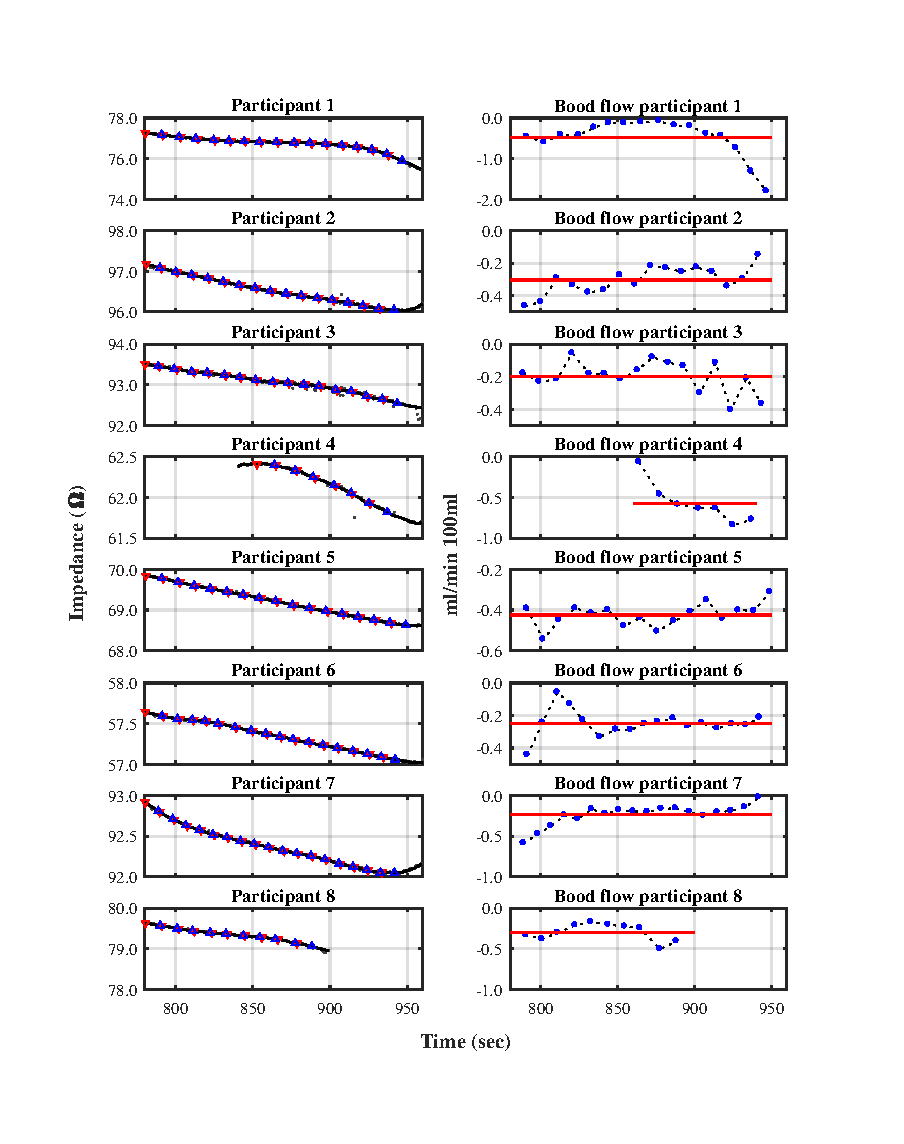
\includegraphics[width=\textwidth,height=\textheight,keepaspectratio,trim={0.5cm 0cm 0cm 1cm},clip]{figure_vop_11}    
	\caption[Blood flow calculated from partial arterial occlusion for every 10 beats]{The figure on the left shows the change of impedance during partial arterial occlusion (\SIrange{780}{960}{\second}). The dots shows the valley points synchronised with the heart cycle. The dark line represents the smoothed data that used to calculate blood flow. The red marker indicates the initial data point $R_{B1}$ and the blue one $R_{B2}$. On the rights, the blood flow in \si{\bfv} for the data points between each marker. The red line indicates the mean of the data points.}
	\label{fig:blood_flow:arterial_occlusion}
\end{figure}

The table \ref{tbl:blood_flow:region4} shows the statistics of the measurements. The data indicated that the average blood flow during the arterial occlusion was \SI{-0.356(0147)}{\bfv}. When compared to the VOP flow, it is considerably larger. Participant 1 depicted the greatest blood flow \SI{-2.260}{\bfv} because of the slope change nearly the end of the experiment

\begin{table}[!htpb]
	\caption{Statistics of the blood flow calculated during partial arterial occlusion. All the numbers are in blood flow units \si{\bfv}, except the column size that is the magnitude of sample.}
	\label{tbl:blood_flow:region4}
	\centering
	\begin{tabular}
		{
			l
			c
			c
			S[table-format=1.3]@{\,\( \pm \)\,}S[table-format=1.3] %Format for Z+-std 
			c
			c
		}
		\toprule
		& \multirow{2}{*}{\textbf{Size}} 
		& \textbf{Median} 
		& \multicolumn{2}{c}{\textbf{Mean}} 
		& \textbf{Max} 
		& \textbf{Min} \\
		& 
		& \small{\si{[\bfv]}} 
		& \multicolumn{2}{c}{\small{\si{[\bfv]}}} 
		& \small{\si{[\bfv]}} 
		& \small{\si{[\bfv]}} \\\midrule
		Participant 1 & 17 & -0.414 & -0.582 & 0.630 & -0.080 & -2.260 \\ 
		Participant 2 & 16 & -0.296 & -0.304 & 0.084 & -0.150 & -0.466 \\ 
		Participant 3 & 17 & -0.182 & -0.199 & 0.093 & -0.056 & -0.403 \\ 
		Participant 4 & 8  & -0.611 & -0.568 & 0.236 & -0.068 & -0.843 \\ 
		Participant 5 & 17 & -0.410 & -0.400 & 0.116 & -0.004 & -0.546 \\ 
		Participant 6 & 18 & -0.249 & -0.247 & 0.078 & -0.057 & -0.443 \\ 
		Participant 7 & 18 & -0.201 & -0.237 & 0.129 & -0.022 & -0.586 \\ 
		Participant 8 & 11 & -0.302 & -0.317 & 0.118 & -0.171 & -0.507 \\ 
\bottomrule
	\end{tabular} 
\end{table}


%%********************************** % Section 7.2.3 ******************************************
\subsection{Comparative change of blood flow between venous and partial arterial}
\label{section occlusion 2.3}
Figure \ref{fig:iPG_flow_comparative} compares the change of blood flow between venous and partial arterial occlusion. As the chart indicates, all the participants experienced an increase in blood flow when the second occlusion took place. Indeed, the numeric value indicates how much the blood flow increased between both measurements. In the plot, the negative symbol of the data collected in sections \ref{section occlusion 2.1} and \ref{section occlusion 2.3} was suppressed since it expresses direction of the blood flow only. These changes of blood flow were expected as the rate of change of impedance during PAO was considerably larger, as displayed in figures \ref{fig:venous occlusion change} and \ref{fig:arterial occlusion change}. 

In general, the blood flow in all the participants increased nearly two times (\num{2.05(064)}). In average the blood flow increased from \SI{0.174(0042)}{\bfv} during venous occlusion to a mean of \SI{0.356(0147)}{\bfv} in partial arterial occlusion. Partakers 1 and 4 experienced the greatest change of blood flow because of sharp changes in impedance during the measurement. In previous sections was discussed the effect of motion in the study that may cause some of these sudden changes of impedance. On the other hand, participant 2 described the least change of blood flow where only increased 1.2 times. \mynote{Find an explanation of why the blood flow increased and discuss it from the physiological point of view}

\begin{figure}[!htpb]
	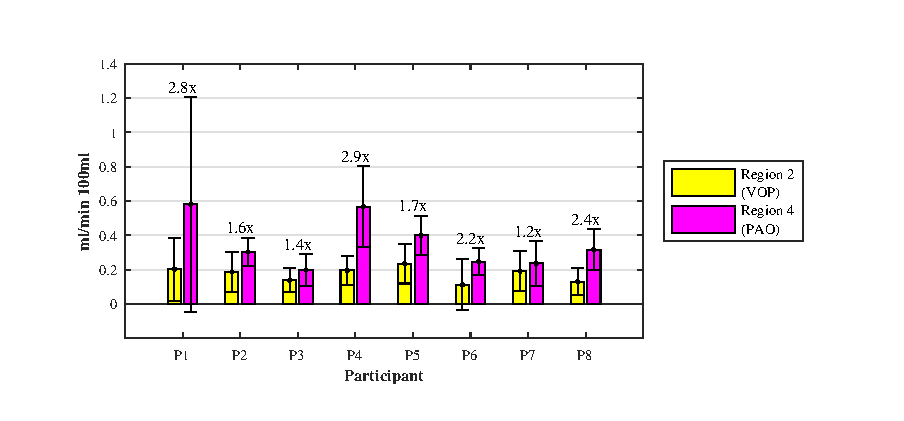
\includegraphics[width=\textwidth,clip]{figure_vop_12}    
	\caption[Comparison of the change of blood flow during venous and partial arterial occlusion]{Comparison of the change of blood flow during venous and partial arterial occlusion. The yellow marker indicated the blood flow during venous occlusion and the magenta the one from partial arterial occlusion. The number indicates the difference in times between both flows.}
	\label{fig:iPG_flow_comparative}
\end{figure}


\section{Conclusions}
\label{section occlusion 3}
The iPG device was able to detect changes as the volume of the forearm change by the effect of the constriction of the upper arm. Clearly, the impedance decreased during venous and partial occlusion. However, during total occlusion there was not a clear trend on the change of impedance. In average from the maximum to the minimum point, the impedance during VOP varied in a \SI{0.658(0230)}{\percent}. On the other hand, all along PAO the impedance changed in \SI{1.13(0482)}{\percent}. In comparison, during total occlusion the impedance slightly went up or down, in average the change was well below the other occlusions around \SI{0.250(0446)}{\percent}. 

The analysis also showed that the acceleration during the first 10 heartbeats is greater than the rest. During these heartbeats, the change of impedance was around \SI{-0.0063(00037)}{\Omega \per \second} for venous occlusion, quite closely partial arterial occlusion was about \SI{-0.0074(00037)}{\Omega \per \second}, and total occlusion was \SI{-0.0027(00052)}{\Omega \per \second}. 

Translating these impedance changes into blood flow resulted in two different values. During VOP the blood flow was about \SI{0.174(0042)}{\bfv}. Interestingly, all along PAO the estimated blood flow doubled, it went up to \SI{0.356(0147)}{\bfv}. In general, creating a partial arterial occlusion at mid-point between diastolic and systolic pressure, folded the blood flow calculated. \mynote{Verify if this is caused by a physiological change of just if there is an error in the calculation during partial arterial} 

%********************************** %Nomenclatures in chapter  **************************************
\nomenclature[z-PAO]{PAO}{Partial arterial occlusion}